\addchap{Fachschaftsrat}

\minisec{Was ist der FSR?}

\begin{wrapfigure}{r}{6cm}\ \\[-1cm]
\flushright
\includegraphics[width=\linewidth]{img/fsr_logo}
\end{wrapfigure}

Der Fachschaftsrat ist deine Vertretung auf Fakultätsebene.
Er wird jährlich gewählt und besteht zur Zeit aus 17 Studenten der Informatik und Medieninformatik.
Als gewähltes Gremium können wir deine Interessen bei den zuständigen Stellen vortragen und so das Studium angenehmer machen.
Neben deiner Vertretung kümmern wir uns um viele weitere Belange.

\minisec{Was wir machen}
Der FSR ist zentrale Anlaufstelle bei Problemen mit dem Studium.
Um es gar nicht so weit kommen zu lassen, unterstützen wir dich im Studium so gut wie es geht.
So sammeln wir alte Prüfungen und Protokolle von Komplexprüfungen und stellen sie für dich online.
Damit die Qualität der Lehre weiter verbessert wird, kümmert sich der FSR um die Evaluation der einzelnen Vorlesungen.
Um dir einen guten Einstieg zu ermöglichen, organisieren wir eine Woche lang und nur für dich und deine Kommilitonen die Erstsemestereinführung.

Jedes Jahr gibt es natürlich die obligatorische Weihnachtsfeier.
Wenn es dann wieder wärmer wird, ist es Zeit für die Grillabende oder ein Sportturnier. \\
Außerdem veranstaltet der FSR regelmäßig Spieleabende mit Brett-, Karten- und digitalen Spielen in der Fakultät.

\minisec{Verleih}
Der FSR bietet für alle Studenten der TU Dresden verschiedene Geräte und Materialien zum ausleihen an. Ausgeliehen werden können unter anderem verschiedene Raspberry Pis, eine Oculus Rift und Lego Mindstorms.
 Wenn ihr etwas ausleihen wollt, dann bringt bitte beim ersten mal euren Personalausweis mit, damit wir auch einen Leihschein ausstellen können. 
Die Liste der auszuleihenden Gegenstände und die Verleihordnung findet man unter \link{https://www.ifsr.de/service:leihen}.

\minisec{Wir brauchen DICH}
WE WANT YOU TO JOIN THE FSR.
Demokratie lebt vom Mitmachen.
Im Gegensatz zur großen Bundesrepublik ist Demokratie an der Uni direkt, mit niedrigen Hürden verbunden und erfolgreich.
Damit das so bleibt, brauchen wir dich im FSR.
Es kann nur so gut gearbeitet werden, wie motivierte FSRlinge da sind.
Studentenvertretung ist, was ihr daraus macht.

\begin{wrapfigure}{l}{7cm}
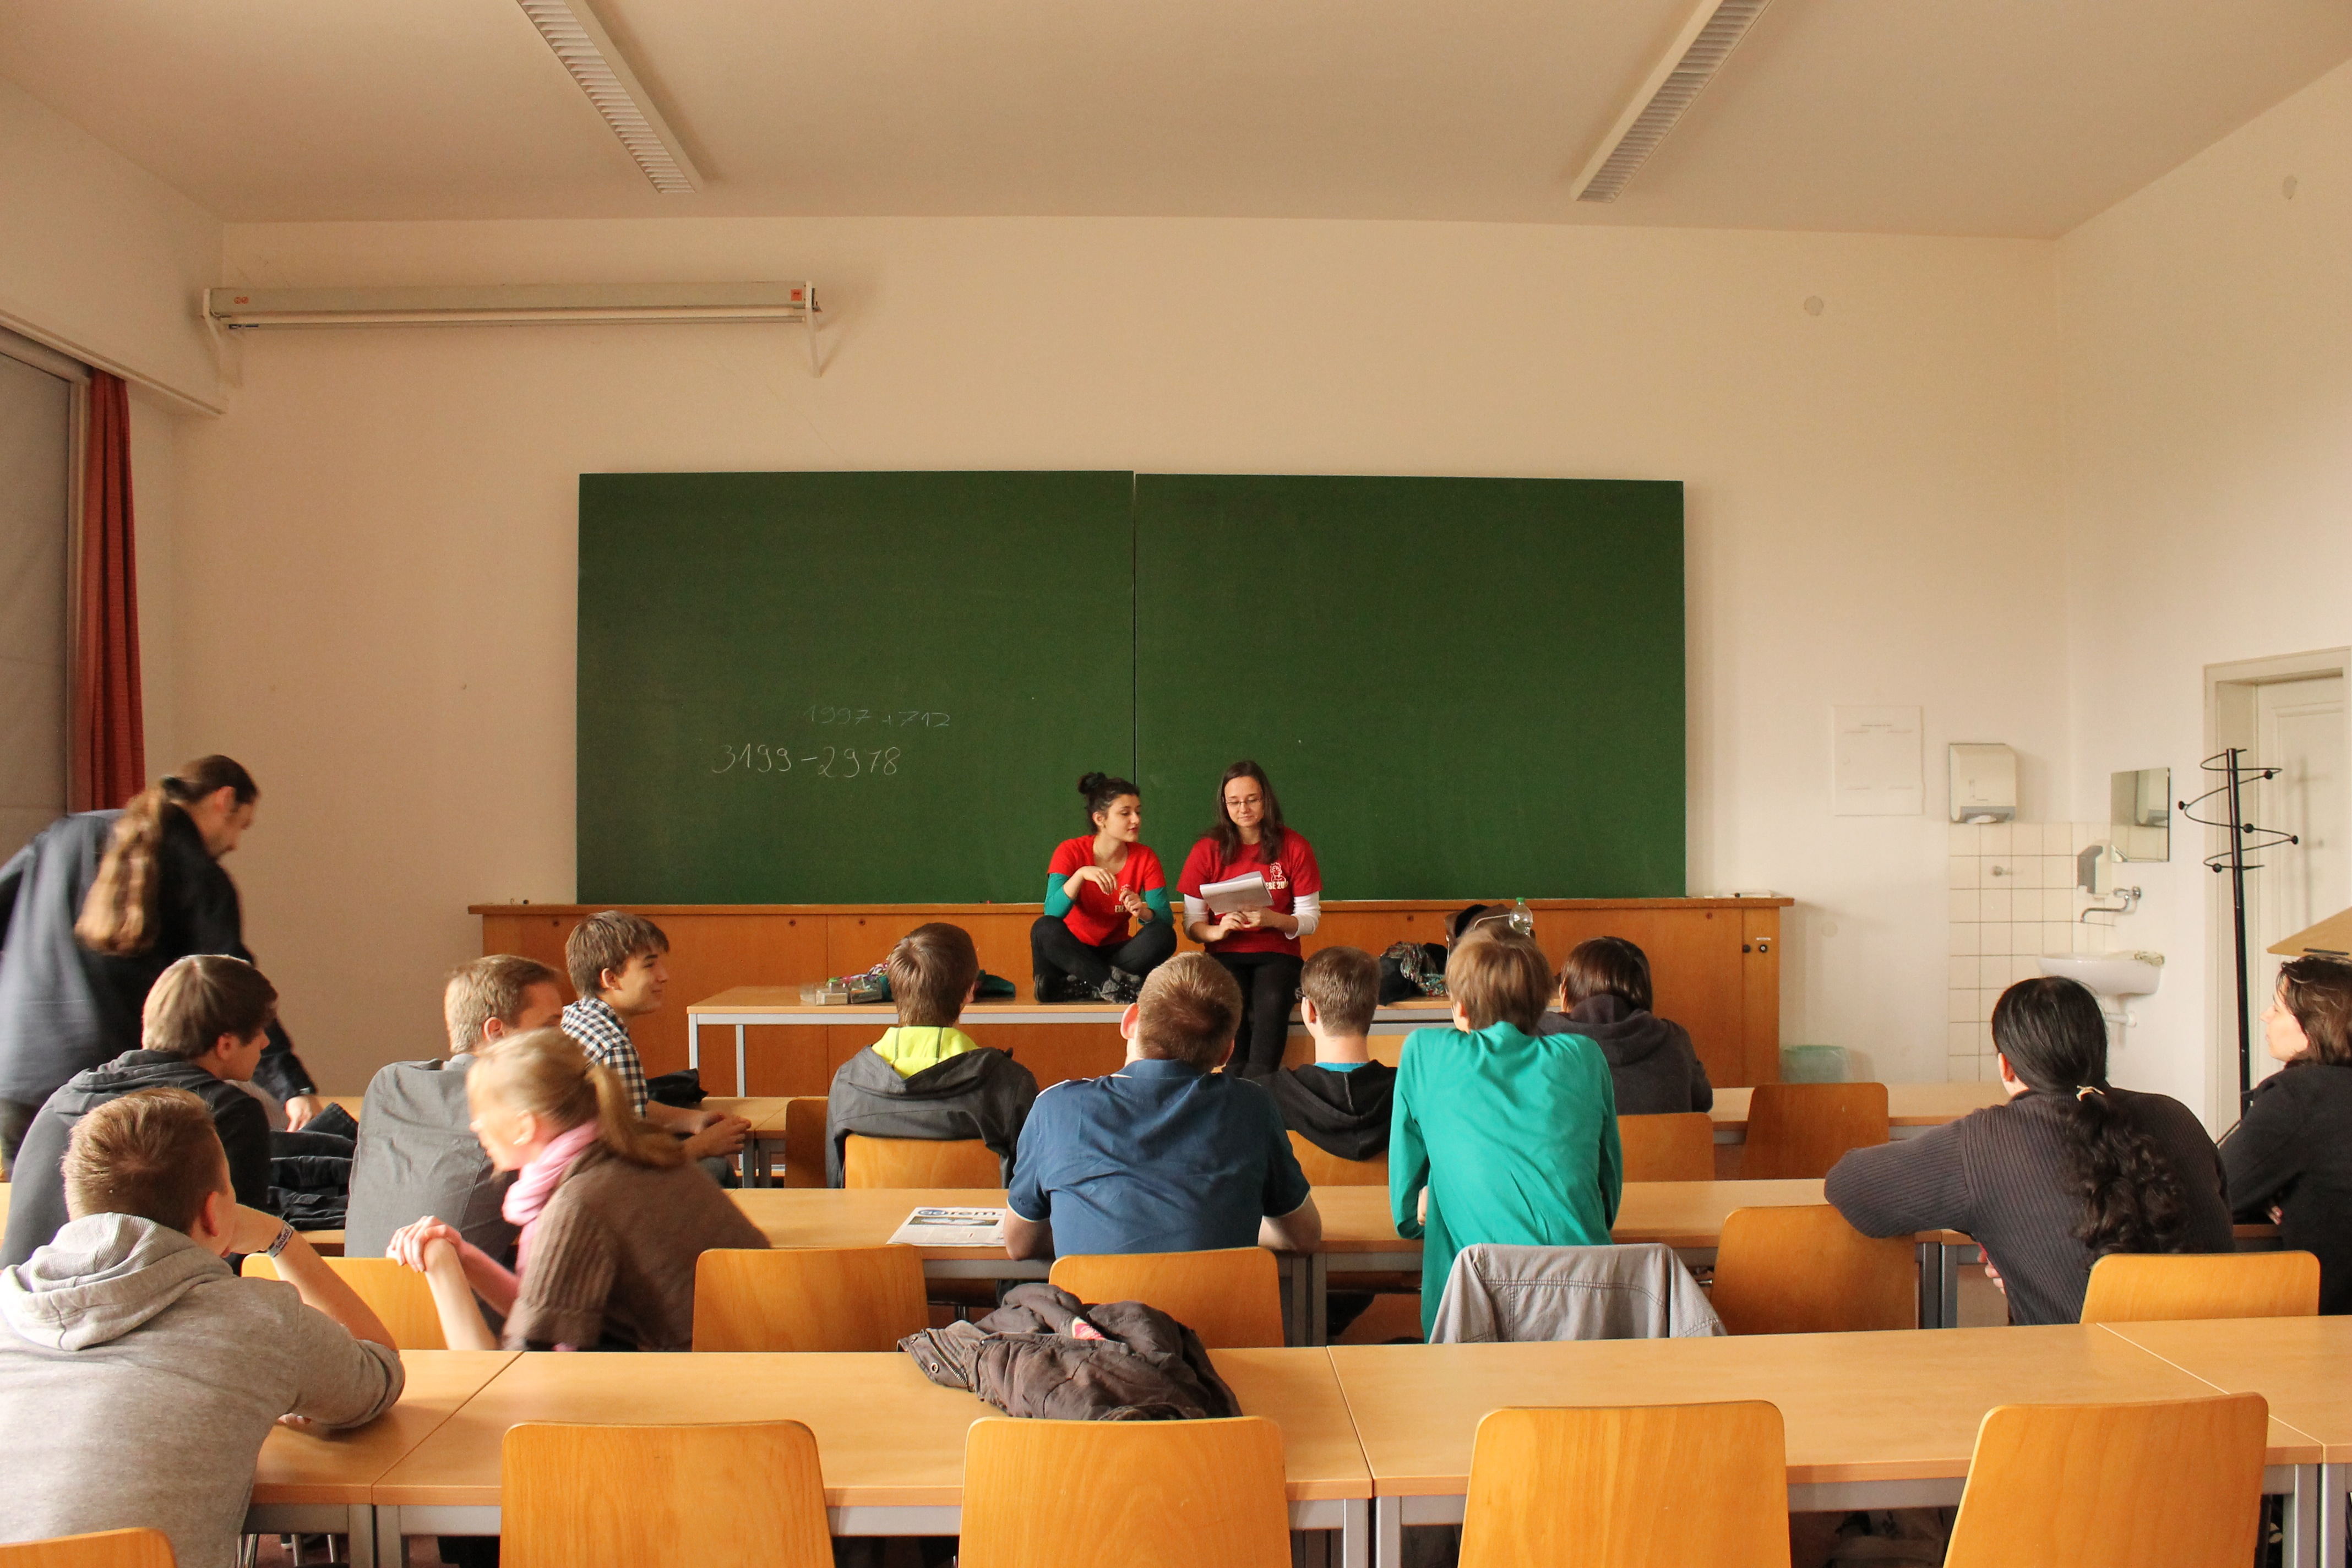
\includegraphics[width=\linewidth]{img/ese2013/tutorium.jpg}
\end{wrapfigure}

GEH WÄHLEN.
Auch wer sich nicht selbst zur Wahl aufstellen lassen will, kann was für seine Fachschaft tun.
Deine Stimme gibt dem FSR Rückhalt bei schwierigen Entscheidungen.

Wir suchen auch immer Organisationstalente für einzelne Veranstaltungen wie die Sporttuniere oder die Lange Nacht der Wissenschaften.
Wenn du dich also nicht das ganze Jahr lang offiziell gewählt engagieren willst, kannst du auch als sogenanntes assoziiertes Mitglied jederzeit mithelfen, die Rahmenbedingungen des Studiums an unserer Fakultät zu verbessern.

\minisec{Kontakt}
Jeden Montagabend treffen wir uns um 18:30 Uhr im großen Ratssaal (APB 1004), um unter anderem über verschiedene Aktionen, sei es ESE, Lehrevaluation, Sporttuniere aber auch über Probleme und Entwicklungen an der Fakultät bzw. Universität zu diskutieren und uns zu engagieren.
Du bist dabei herzlichst eingeladen, denn die Sitzung ist für alle öffentlich!
Den Rest der Zeit sind wir eigentlich immer im Büro im Erdgeschoss des Fakultätsgebäudes aufzufinden.

Wo: APB E017 \\
Sitzung: immer montags 18:30 Uhr \\
E-Mail: fsr@ifsr.de \\
Web: www.ifsr.de \link{https://www.ifsr.de/}

\newcommand{\fsrler}[5]{% filename, vorname, nachname, username, studiengang
\fbox{\begin{minipage}{.25\linewidth}
    \centering\vspace{.8em}
    \includegraphics[width=.8\linewidth]{img/fsr/#1}\\[.6em]
    {\Large #2}\\[.2em]
    {\large#3}\\[.5em]
    \textit{\small #5}\\
    \texttt{\small #4@ifsr.de}\\[-.1em]\ 
\end{minipage}}\hspace{3em}%
}

\fsrler{anita.jpg}{Anita}{Grützner}{anita}{Diplom INF 7. Sem.}
\fsrler{ben.jpg}{Ben}{Kosmann}{kosmann}{Bachelor INF 7. Sem.}
\fsrler{felix.jpg}{Felix}{Döring}{felix}{Diplom INF 5. Sem.}\\[1em]

\fsrler{franz.jpg}{Franz}{Schumann}{franz}{Bachelor MINF 5. Sem.} % -Wilhelm macht Dinge kaputt, sorry :D
\fsrler{ian.jpg}{Ian}{List}{ian}{Bachelor INF 6. Sem.}
\fsrler{jonas.jpg}{Jonas}{Wielicki}{jonas}{Bachelor INF 7. Sem.}\\[1em]

\fsrler{julius.jpg}{Julius}{Gonsior}{julius}{Diplom INF 6. Sem.}
\fsrler{katja.jpg}{Katja}{Linnemann}{linnemann}{Diplom INF 5. Sem.}
\fsrler{lars.jpg}{Lars}{Engeln}{lars}{Master MINF 3. Sem.}\\
%
\fsrler{marcel.jpg}{Marcel}{Rösler}{marcel}{Diplom INF 7. Sem.}
\fsrler{marc.jpg}{Marc}{Satkowski}{satkowski}{Diplom INF 7. Sem.}
\fsrler{nico.jpg}{Nico}{Westerbeck}{westerbeck}{Diplom INF 5. Sem.}\\[1em]

\fsrler{philipp.jpg}{Philipp}{Heisig}{heisig}{Bachelor MINF 7. Sem.}
\fsrler{sascha.jpg}{Sascha}{Peukert}{sascha}{Diplom INF 8. Sem.}
\fsrler{sebastian.jpg}{Sebastian}{Mielke}{mielke}{Master INF 1. Sem.}\\[1em]

\fsrler{schrader.jpg}{Sebastian}{Schrader}{schrader}{Diplom INF 11. Sem.}
\fsrler{simon.jpg}{Simon}{Hanisch}{simon}{Master INF 1. Sem.}
\fsrler{questionmark.png}{Du}{vielleicht?}{dein\_name}{Erstes Semester}\\

\ 
\thispagestyle{empty} %keine Seitenzahl
\AddToShipoutPicture*{\put(0,0){%
\parbox[b][\paperheight]{\paperwidth}{%
\vfill
\centering
\includegraphics[width=\dimen107,height=\dimen108,keepaspectratio]{img/spieleabend.png}%
\vfill
}}}
